\documentclass[UTF-8, a4paper, 12pt]{ctexart}

\usepackage[left=1in,right=1in,top=1.00in,bottom=1.00in]{geometry}% 页边距
\usepackage[colorlinks,linkcolor=blue,anchorcolor=blue,citecolor=green,CJKbookmarks=True]{hyperref}
\usepackage{CJK,CJKnumb}
\usepackage{indentfirst}        % 首行缩进宏包
\usepackage{latexsym,bm}        % 处理数学公式中和黑斜体的宏包
\usepackage{amsmath,amssymb}     % AMSLaTeX宏包 用来排出更加漂亮的公式
\usepackage{graphicx}
\usepackage{cases}
\usepackage{pifont}
\usepackage{txfonts}
\usepackage{subfigure}
\usepackage{pdfpages}
\usepackage{listings}
\usepackage{xcolor}
\usepackage[subfigure]{tocloft}     % 模板中用了subfigure,不加此选项会产生冲突
\usepackage{inconsolata}
\CTEXsetup[format={\Large\bfseries}]{section}%设置章标题字号为Large,居左
\zihao{-4}\linespread{1.5}\selectfont
\renewcommand{\theequation}{\arabic{section}-\arabic{equation}}
\renewcommand{\thefigure}{\arabic{section}-\arabic{figure}}
%\renewcommand{\thefigure}{\thechapter-\arabic{figure}}
\renewcommand{\cftsecleader}{\cftdotfill{\cftdotsep}}
\renewcommand\contentsname{{\qquad\qquad\qquad\qquad\qquad\qquad 目\quad 录}}
\newcommand{\song}{\CJKfamily{song}}    % 宋体   (Windows自带simsun.ttf)
\renewcommand{\abstractname}{\textbf{\large {摘\quad 要}}} %更改摘要二字的样式

%%%%%%%%%%%%%%%%%%%%%%%
% -- text font --
% compile using Xelatex
%%%%%%%%%%%%%%%%%%%%%%%
% -- 中文字体 --
%\setCJKmainfont{Microsoft YaHei}  % 微软雅黑
%\setCJKmainfont{YouYuan}  % 幼圆
%\setCJKmainfont{NSimSun}  % 新宋体
%\setCJKmainfont{KaiTi}    % 楷体
%\setCJKmainfont{SimSun}   % 宋体
%\setCJKmainfont{FangSong}   % 仿宋
%\setCJKmainfont{SimHei}   % 黑体
 
% -- 英文字体 --
%\setmainfont{Times New Roman}
%\setmainfont{DejaVu Sans}
%\setmainfont{Latin Modern Mono}
%\setmainfont{Consolas}
\setmainfont{CMU Serif}


%%%%%%%%%%%%%%%%%%%%%%%
%  设置水印
%%%%%%%%%%%%%%%%%%%%%%%
%\usepackage{draftwatermark}         % 所有页加水印
%\usepackage[firstpage]{draftwatermark} % 只有第一页加水印
%\SetWatermarkText{Copyright(C) 2021. by HU S K}           % 设置水印内容
% \SetWatermarkText{\includegraphics{fig/ZJDX-WaterMark.eps}}         % 设置水印logo
%\SetWatermarkLightness{00.9}             % 设置水印透明度 0-1
%\SetWatermarkScale{0.4}                   % 设置水印大小 0-1
%%%%%%%%%%%%%%%%%%%%%%%




%%%%%%%%%%%%%%%%%%%%%%%%%%%%%%%%%%%%%%%%%%%
%用来设置附录中代码的样式
% 头文件
%%%%%%%%%%%%%%%%%%%%%%%%%%%%%%%%%%%%%%%%%%%
\usepackage{listings} 
\usepackage{fontspec}
\setmonofont{Consolas}
%\begin{lstlisting}[
%	language = matlab, numbers=left, 
%	numberstyle=\tiny,keywordstyle=\color{blue!70},
%	commentstyle=\color{red!50!green!50!blue!50},frame=shadowbox,
%	rulesepcolor=\color{red!20!green!20!blue!20},
%	basicstyle=\ttfamily,
%	]
%	
%\end{lstlisting}



\title{\bfseries \Huge  }
\author{}
\date{}

\begin{document}
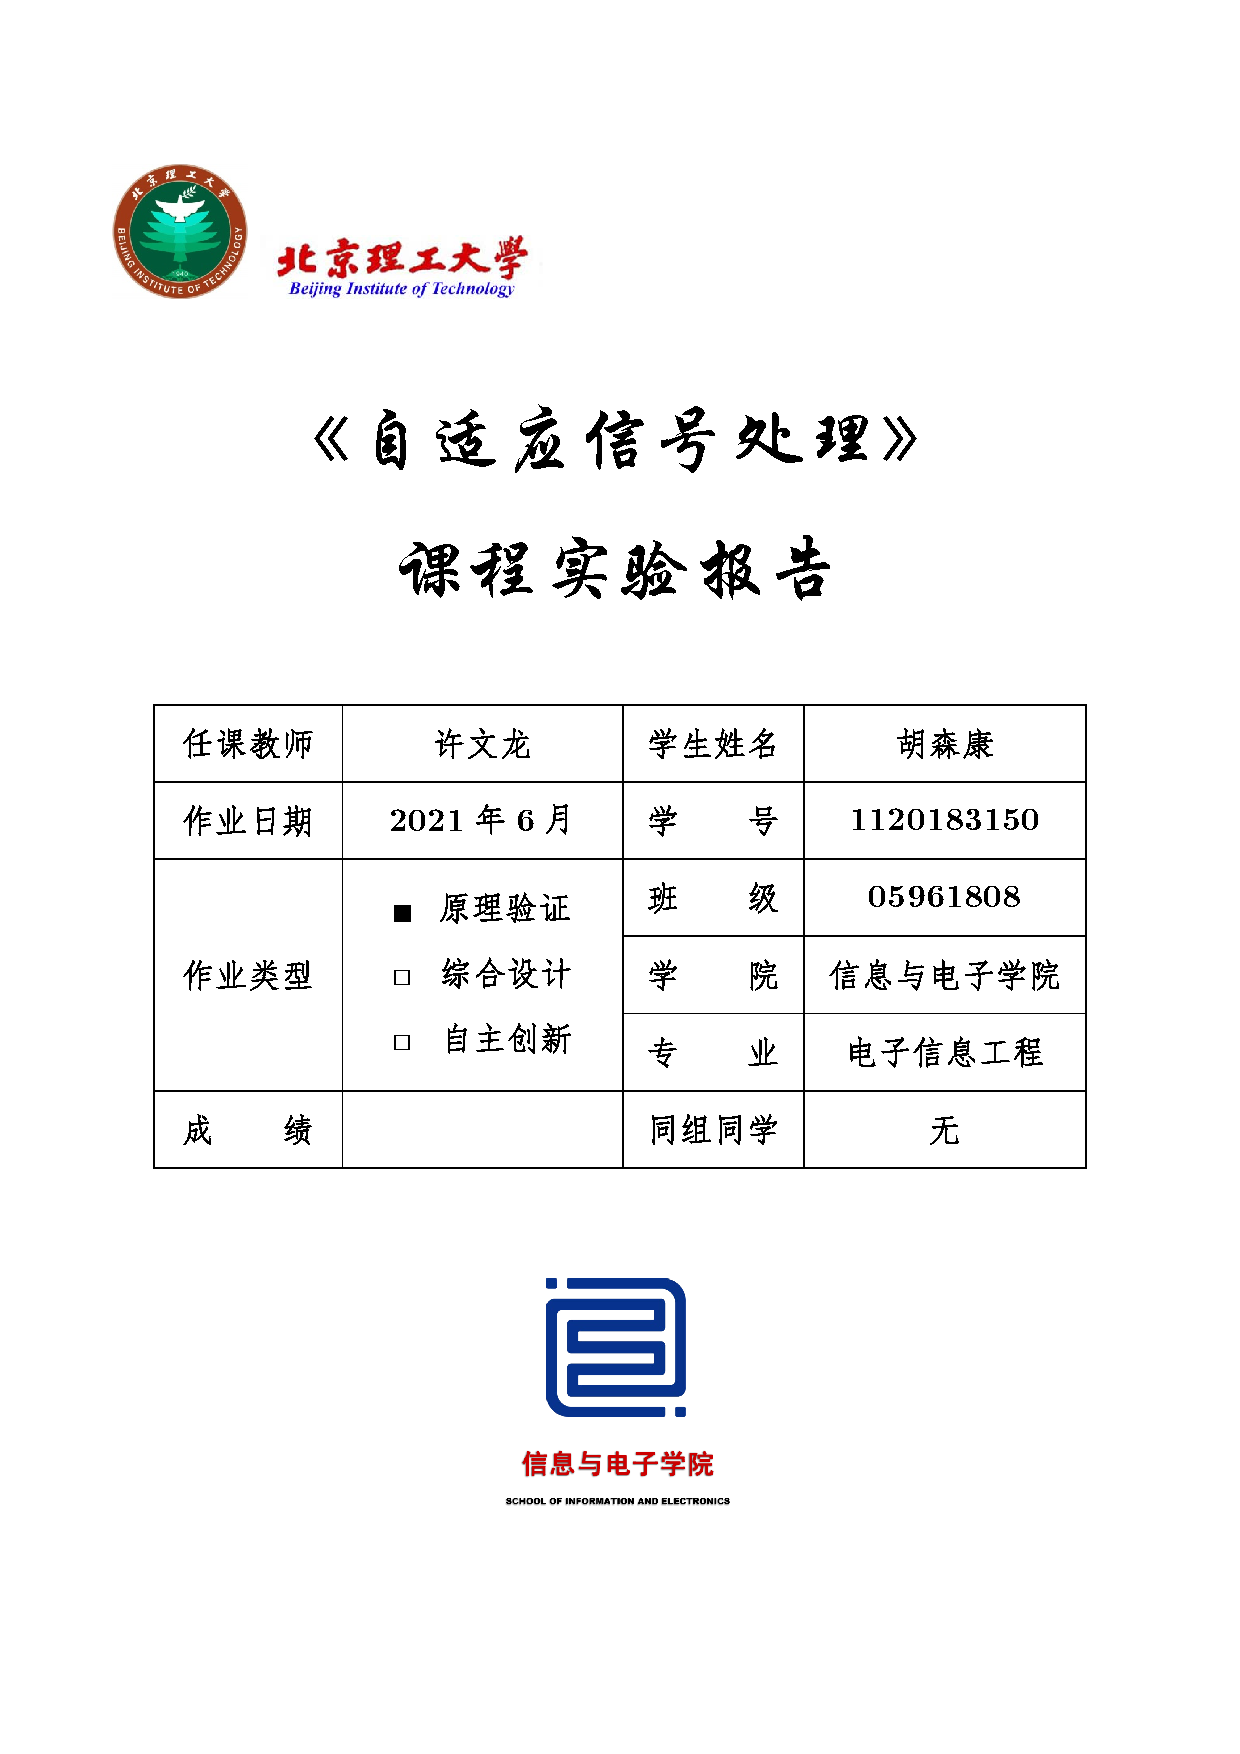
\includepdf[pages={1}]{coverpage.pdf} %% 插入pdf

%\maketitle

%\thispagestyle{empty}
%\newpage
%\thispagestyle{empty}


     

     
%\thispagestyle{empty}       %本页不显示页码
%\newpage                    %分页
\tableofcontents\thispagestyle{empty}
\newpage
\setcounter{page}{1}        %从下面开始编页,页脚格式为导言部分设置的格式



\section{第3章 最小均方(LMS)算法 26题}
\subsection{Question Statement}

在系统辨识问题中,假设输入信号为四进制QAM信号,并具有下列形式
\begin{equation}
    x(k)=x_{re}(k)+jx_{im}(k)
\end{equation}
其中,$x_{re}(k)$和$x_{im}(k)$为随机产生的$\pm 1$。未知系统表示为
\begin{equation}
    H(z)=0.32+0.21j+(-3+0.7j)z^{-1}+(0.5-0.8)z^{-2}+(0.2+0.5j)z^{-3}
\end{equation}
自适应滤波器也是一个三阶FIR滤波器,加性噪声是方差为$\sigma_n^2=0.4$的零均值高斯白噪声。采用复数LMS算法,选取适当的$\mu$值,运行20次实验,画出平均学习曲线。

\subsection{Solution}

We have the plots:
\begin{figure}[htbp]
    \centering
    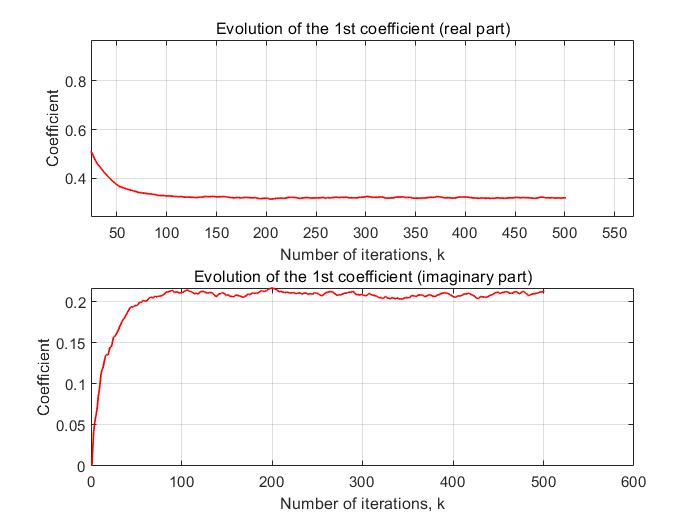
\includegraphics[width=13cm]{3.26/mu1_coefficient.jpg}
    \caption{Evolution of the 1st coefficient (real and imaginary part), $\mu=0.1$}
\end{figure}
\begin{figure}[htbp]
    \centering
    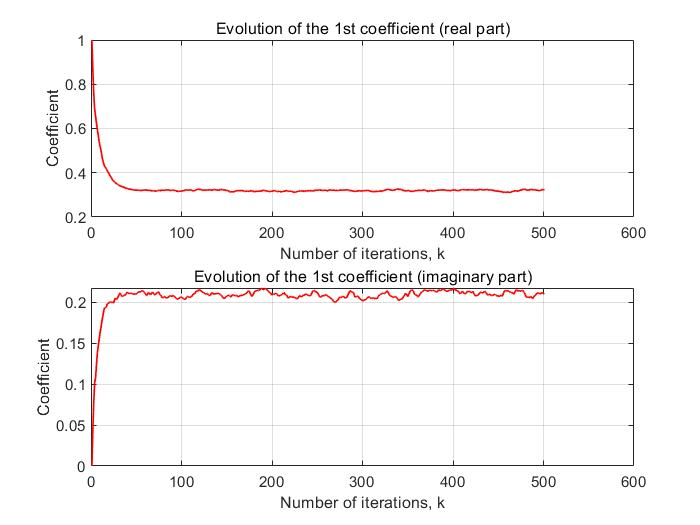
\includegraphics[width=13cm]{3.26/mu2_coefficient.jpg}
    \caption{Evolution of the 1st coefficient (real and imaginary part), $\mu=0.2$}
\end{figure}

\begin{figure}[htbp]
    \centering
    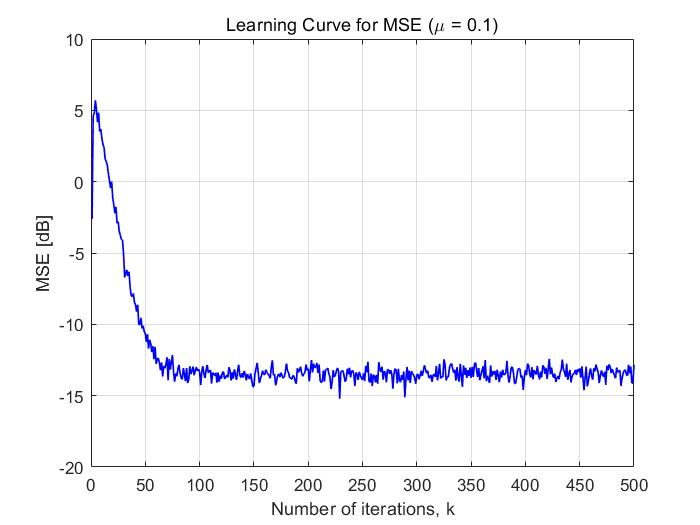
\includegraphics[width=13cm]{3.26/mu1_curve.jpg}
    \caption{Learning Curve for MSE, $\mu=0.1$}
\end{figure}

\begin{figure}[htbp]
    \centering
    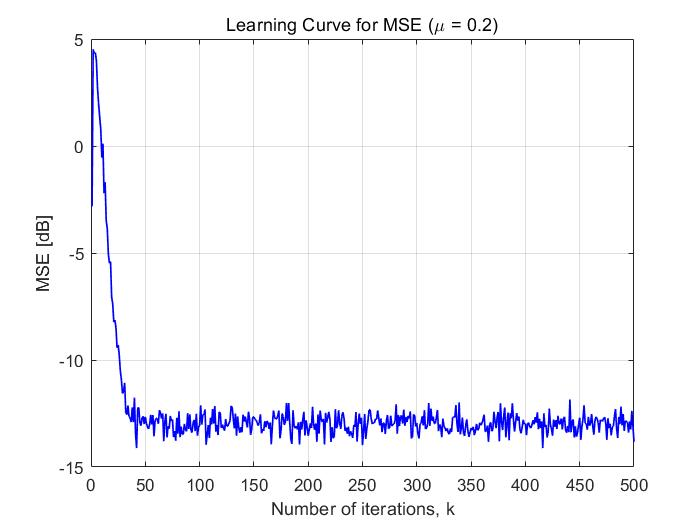
\includegraphics[width=13cm]{3.26/mu2_curve.jpg}
    \caption{Learning Curve for MSE, $\mu=0.2$}
\end{figure}

\newpage

We choose  $\mu=0.1$ and run this program 20 times ,and we have the average learning curve (Figure (\ref{av})) for MSE:

\begin{figure}[htbp]
    \centering
    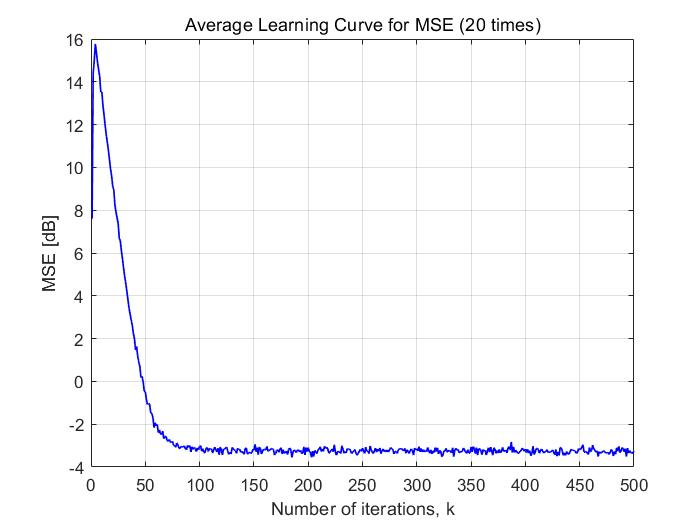
\includegraphics[width=14cm]{3.26/average.jpg}
    \caption{Average Learning Curve for MSE (20 times) }
    \label{av}
\end{figure}

\newpage
\section{第4章 基于LMS准则的算法 13题}
\subsection{Question Statement}
采用符号误差算法辨识7阶时变未知系统,其系数为一阶马尔可夫过程,并且$\lambda_{\boldsymbol{w} }=0.999$,$\sigma_{\boldsymbol{w}}^2=0.001$。时变系统乘积系数的初始值为
\begin{equation}
    \boldsymbol{w}_{o}^{\mathrm{T}}=\left[0.03490\ -0.011\ -0.06864\ 0.22391\ 0.55686\ 0.35798\ -0.0239\ -0.07594\right]
\end{equation}
输入信号为$\sigma_x^2=7$的高斯白噪声,测量噪声是与输入信号以及$\boldsymbol{n}_{\boldsymbol{w}}(k)$的元素独里、方差为$\sigma_n^2=0.01$的高斯白噪声。若$\mu=0.01$,对上述实验进行仿真,并得到超量MSE的测量值。
\subsection{Solution}
We have the plots:
\begin{figure}[htbp]
    \centering
    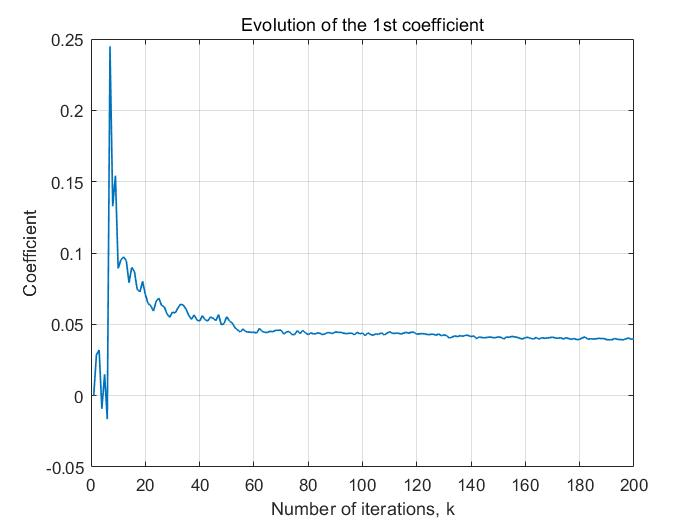
\includegraphics[width=13cm]{4.13/f1.jpg}
    \caption{Evolution of the 1st Coefficient}
\end{figure}



\begin{figure}[htbp]
    \centering
    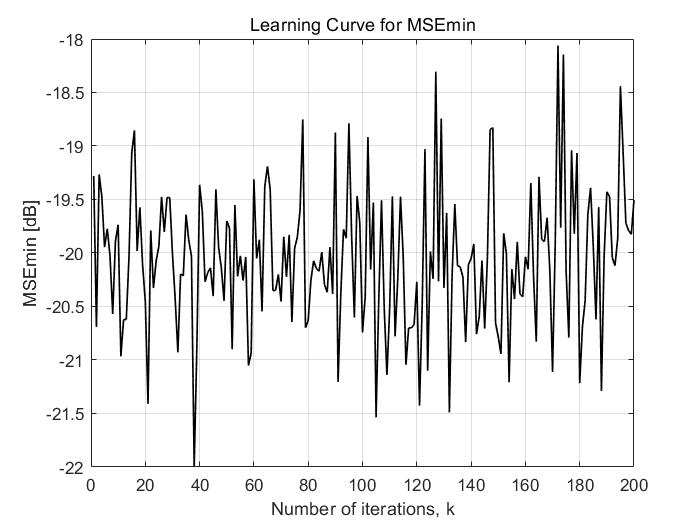
\includegraphics[width=13cm]{4.13/f2.jpg}
    \caption{Learning Curve for MSEmin}
\end{figure}

\begin{figure}[htbp]
    \centering
    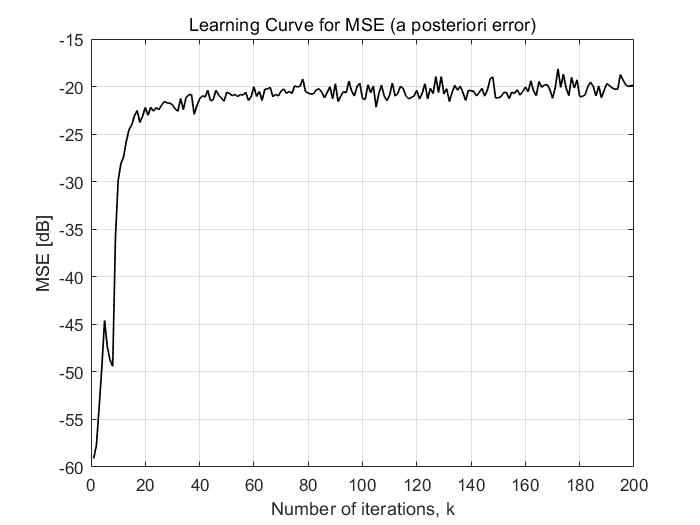
\includegraphics[width=13cm]{4.13/f3.jpg}
    \caption{Learning Curve for MSEmin (A Posteriori Error)}
\end{figure}

\newpage

And we get the excess MSE by measuring the plot, the excess MSE approximately is 1.2589.

\end{document}